\chapter{Stokes Equation}
\label{cha:stokes-equation}

\section{Problem Overview}
\label{sec:problem-formulation}

A fundamental problem in Solid Earth Sciences is the solution of
Stokes equation for the incompressible creeping flow of a highly
viscous fluid.
\begin{align}
-\div\eta(\grad\vec{v} + \grad\vec{v}^{T}) + \grad p &= \vec{f}\\ 
\div \vec{v} = 0 & 
\end{align}
where $\vec{v}$ is the fluid velocity field,  $p$ is the pressure
which acts to enforce the incompressibility constraint, $\eta$ is the
fluid viscosity and $\vec{f}$ are body forces (usually buoyancy) that
drive flow.

Stokes Equation is computationally and mathematically more challenging
to solve than Poisson's equation in Chapter
\ref{cha:poiss-equat-unit}, particularly for non-constant viscosity.
To begin with, Stokes is a coupled system of PDE's for $\vec{u} =
(\vec{v},p)$ which in finite elements we can capture by describing
$\vec{u}$ as a mixed-element on a mixed finite element function space.
The proper choice of elements for $\vec{v}$ and $p$ is critical for
stability and solution of this problem.  Elman et
al. \cite{elman_finite_2005} provide a good discussion of the issues
for the isoviscous case and May and Moresi \cite{may_preconditioned_2008} provides
important extensions and tests of a large range of iterative solvers
for the variable viscosity case.

Here we will just illustrate the basic isoviscous problem with a range
of direct and iterative solvers that highlight the Fieldsplit block
preconditioners in PETSc \cite{brown_composable_2012} and their
implementation in \TF{}.  While the computational choices required to
solve Stokes efficiently and accurately are more involved
than Poisson,  we will demonstrate that setting the problem up in
\TF{} is a straightforward extension of the problems in Chapter
\ref{cha:poiss-equat-unit}. 

\subsection{Variational forms}
\label{sec:variational-forms}

For this tutorial, we will use a stable ``Taylor-Hood'' element where
velocity is assumed to be a vector valued function with each component
a piecewise quadratic function (i.e.\ for a 2-D problem on triangles
$\vec{v}\in [P_{2}\times P_{2}]$) while the pressure is piecewise
linear ($p\in P_{1}$) such that the entire system $\vec{u}\in \fspace
= [[P_{2}\times P_{2}]\times P_{1}]$.  The variational form of the
(possibly) non-linear problem can be written
\begin{quote}
  \fbox{\parbox{.9\textwidth}{Find $\vec{u}\in \fspace$ such that
      \begin{equation}
         F(\vec{u};\vec{u}_{t}) =0 
      \end{equation}
  for all test functions $\vec{u}_{t}=(\vec{v}_{t},p_{t}) \in\fspace$.}}
\end{quote}
 where $F(\vec{u};\vec{u}_{t}) = F_{\vec{v}} + F_{p}$ with
\begin{align}
         F_{\vec{v}} =  & \int_\Omega \left[\dot{\epsilon}(\vec{v}_{t}):
             2\eta \dot{\epsilon}(\vec{v}_{i}) -
             p_{i}\div\vec{v}_t  - \vec{v}_{t} \cdot\vec{f} \right]d\vec{x}  \\
 F_{p} =& -\int_\Omega p_t\div\vec{v}_{i} d\vec{x}
\end{align}
(after some algebra and integration by parts). Here
\begin{equation}
  \label{eq:19}
  \dot{\epsilon}(\vec{v}) = \frac{1}{2}
  \left(
\grad\vec{v} + \grad\vec{v}^{T}
  \right)
\end{equation} is the strain-rate tensor (i.e. the symmetric part of
deformation tensor $\grad\vec{v}$).   

The weak form of the residual in UFL looks quite similar
\begin{lstlisting}[style=UFL]
Fv = (inner(sym(grad(v_t)),2.*eta*sym(grad(v_i)))
    - p_i*div(v_t) - inner(v_t,f)*dx  
Fp = -p_t*div(v_i)*dx 

F =  Fv + Fp 
\end{lstlisting}
and the Jacobian
\begin{lstlisting}[style=UFL]
  J = derivative(F,u_i,u_a)
\end{lstlisting}
assembles into the $2\times2$ block system
\begin{equation}
  \label{eq:20}
  J =
  \left[
    \begin{array}{cc}
      K & G \\
      G^{T} & 0\\
    \end{array}
  \right]
\end{equation}

The discrete problem Eq. (\ref{eq:20}),  is the classic Stokes
saddle-point system.  Here we will just scratch the
surface with a simplified MMS solution that implements some basic solution
strategies taken from \cite{elman_finite_2005}.  To fully specify the
problem we need boundary conditions and a forcing function $\vec{f}$. Elman et. al \cite{elman_finite_2005} provide  the
2-D manufactured solution 
\begin{align}
  \vec{v}_{x}(x,y) =& 20xy^{3} \nonumber \\
  \vec{v}_{y}(x,y) =& 5(x^{4} - y^{4})  \label{eq:stokes-mms}
\\
   p(x,y) =& 60x^{2}y - 20y^{3} \nonumber \\
   \vec{f}(x,y) =& \vec{0} \nonumber 
\end{align}
on the domain  $\Omega=[-1,1]\times[-1,1]$ with dirichlet boundary conditions on velocity interpolated from the
analytic solution.  Note: the discrete problem with all dirichlet
conditions on velocity is singular (with a trivial constant null space
for the pressure) and some care needs to be taken with both direct and
iterative solvers to solve this problem accurately.

\section{Solution using \TF}
\label{sec:solution-using-tf}

However, setting this problem up in \TF{} is not
much more difficult than solving the scalar Poisson equation.  The
principal changes from the mms problem \texttt{poisson.tfml} are
\begin{itemize}
\setlength{\itemsep}{0em}
\item We  change the domain from $[0,1]\times[0,1]$ to
  $[-1,1]\times[-1,1]$ (mesh changes to Rectangle)
\item The system now includes two fields for $\vec{v}$ and $p$
\item The field Velocity, is now vector valued and should be in
  $[P_{2}\times P_{2}]$
\item The field Pressure is a scalar in $P_{1}$ with no Boundary
  conditions and a constant null space.
\item Each of the fields will require diagnostics, IC's and BC's
\item The forcing term and boundary conditions just need to be made
  consistent for this MMS problem
\item The non-linear residual needs to change to the above UFL
\end{itemize}

A fully worked out \texttt{tfml} file for this problem using a direct
solver along with a testharness file \texttt{stokes.shml} for running
the convergence test can be
found in \texttt{\$TF\_HOME/share/terraferma/tutorials/stokes/isoviscous/mms/mms\_direct}.
The solution is shown in Figure \ref{fig:stokesMMS}.  Figure
\ref{fig:stokes_convergence}  shows the convergence behavior for both
velocity and pressure and shows larger errors for pressure which
decrease as $h^{2}$ compared to errors for velocity which scale as
$h^{3}$. This plot can be reproduced using
\begin{lstlisting}[style=Bash]
$ cd $TF_HOME/share/terraferma/tutorials/stokes/isoviscous/mms/mms_direct
$ tfsimulationharness --test stokes.shml
\end{lstlisting} %$


\begin{figure}[htbp!]
  \centering
  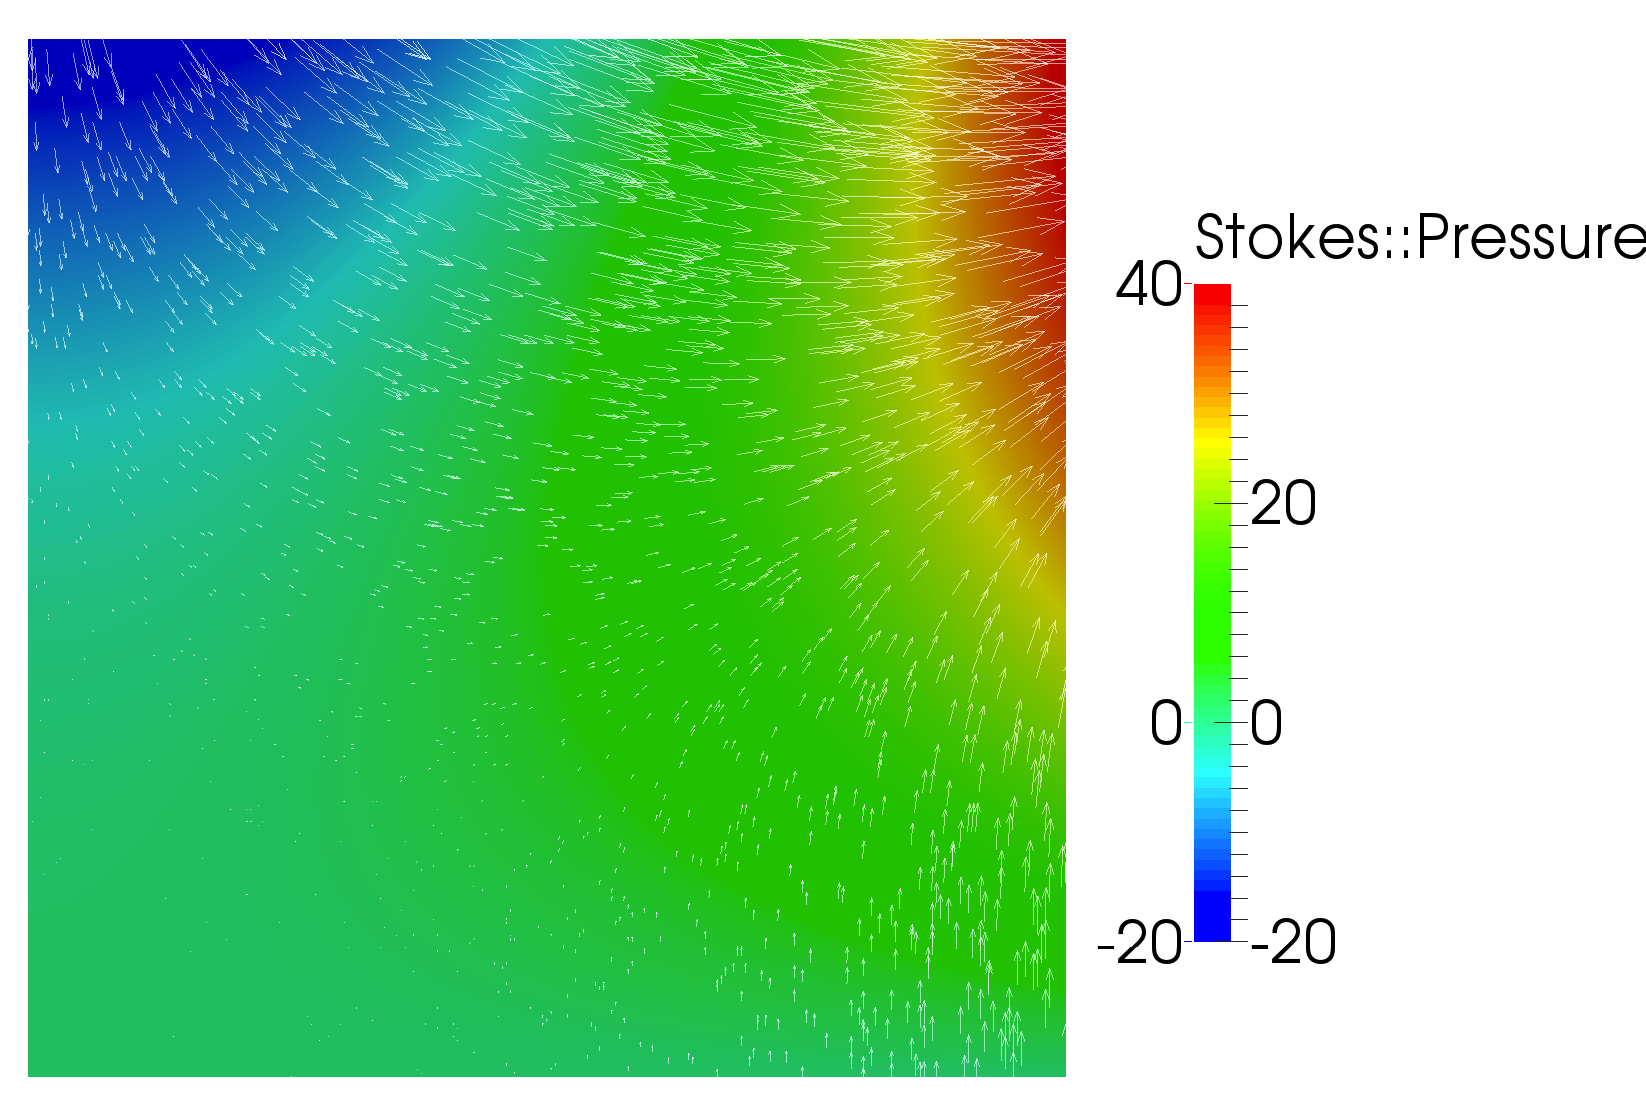
\includegraphics[width=.7\textwidth]{figures/stokes_flow.png}
  \caption{MMS solution of Stokes equation from
    \cite{elman_finite_2005} showing the pressure field in the background color map and the velocity field shown with arrows.}
  \label{fig:stokesMMS}
\end{figure}
\begin{figure}[htbp!]
  \centering
  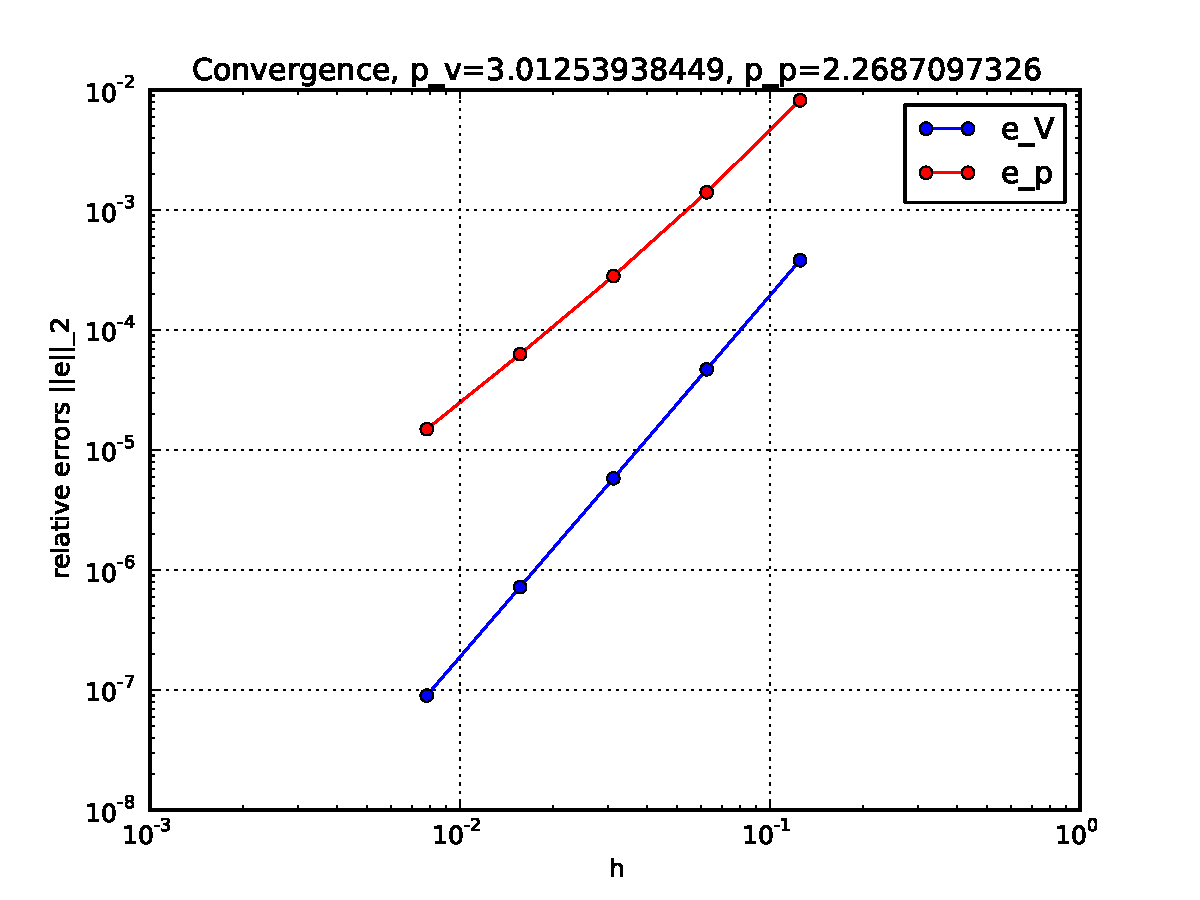
\includegraphics[width=.7\textwidth]{figures/Stokes_convergence.pdf}
  \caption{Convergence behavior of stokes solution for isoviscous
    stokes using P2-P1 ``Taylor-Hood'' mixed elements.}
  \label{fig:stokes_convergence}
\end{figure}

\pagebreak{}

In more detail, the specific steps required to modify the poisson mms
problem to solve Stokes are as follows.
\begin{steps}{Step}
\item Make a new tfml file
  \begin{lstlisting}[style=Bash]
$ mkdir mystokes
$ cd mystokes
$ cp $TF_HOME/share/terraferma/tutorials/poisson/mms/poisson.tfml stokes.tfml
$ diamond stokes.tfml &
  \end{lstlisting}%$
\item \textbf{Change the geometry:} Under \texttt{geometry->Mesh},
  \begin{steps}{step}
  \item Change source from UnitSquare to Rectangle
  \item Set \texttt{lower\_left} to $-1.,-1.$
  \item Set \texttt{upper\_right} to $1.,1.$
  \item Set \texttt{number\_cells} to $32,32$
  \item Set \texttt{diagonal} to \texttt{right/left}
  \end{steps}
\item \textbf{Change io parameters}
  \begin{steps}{step}
  \item Change \texttt{output\_base\_name} to \texttt{stokes}
  \item Change \texttt{visualization->element} to (P2)
  \end{steps}
\item \textbf{Modify System Poisson to System Stokes}
  \begin{steps}{step}
  \item Change the system name to  Stokes (the \texttt{ufl\_symbol}
    remain the same, \texttt{us})
  \item Change the field \texttt{u} to \texttt{Velocity}
    \begin{itemize}{}
    \item change the field name to \texttt{Velocity}
    \item change the \texttt{ufl\_symbol} to \texttt{v}
    \end{itemize}
  \item Modify the velocity field to be vector valued [P2,P2]
    function.   Under \texttt{type (Function)}
    \begin{itemize}{}
    \item Change \texttt{rank} from Scalar to \texttt{Vector}
    \item Set \texttt{element} to P2
    \end{itemize}
  \item Set the velocity Initial Condition to constant $[0.,0.]$
  \item Set the Velocity Boundary conditions to the MMS solution
    \begin{itemize}
    \item Activate a new \texttt{boundary\_condition} under
      \texttt{rank} and name it \texttt{mms}
    \item Set \texttt{boundary\_ids} to \texttt{1 2 3 4} (all boundaries)
    \item Under \texttt{sub\_components (All)} choose \texttt{type (Dirichlet)
        -> python}
    \item Add a new python function to evaluate the velocity boundary
      conditions as a function of $x$ using Equation (\ref{eq:stokes-mms}).
      \begin{lstlisting}[style=Python]
def val(x):
  u = 20.*x[0]*x[1]**3
  v = 5.*(x[0]**4 - x[1]**4)
  return [u,v]
      \end{lstlisting}
    \end{itemize}
  \item \textbf{Check the diagnostics for a vector valued
      velocity}. Just check that only
    \texttt{include\_in\_visualization} and
    \texttt{include\_in\_statistics} are chosen (although feel free to try any
    other option as well)
    \item \textbf{add a new field for Pressure}
      \begin{itemize}
      \item Either create a new Field tab or copy the Velocity tab and
        rename to Pressure
      \item Set the \texttt{ufl\_symbol} to \texttt{p}
      \item Choose \texttt{type (Function)} and
        \begin{itemize}
        \item Set \texttt{rank (Scalar)}
        \item Set \texttt{element (P1)}
        \item Set \texttt{initial\_condition} to a constant (0.0)
        \end{itemize}
      \item \textbf{Set a reference point:}  Stokes with all dirichlet
        BC's for velocity is actually singular allowing an arbitrary
        constant in the pressure.  There are multiple ways in TF to
        remove this singularity.  For direct solvers, we can set  a single reference
        point where the pressure is constrained to be zero. For
        the MMS solution given here, $p=0$ at coordinates $(0.,0.)$.
        To set this point.  Activate the \texttt{reference\_point
          (Point)} tab and set the coordinates to $(0.,0.)$.
      \end{itemize}
  \item \textbf{Set the diagnostics for Pressure}: add \texttt{include\_in\_visualization} and \texttt{include\_in\_statistics}
    % \begin{itemize}
    % \item add \texttt{include\_in\_visualization} and 
    % \item Under \texttt{include\_in\_statistics}
    %   \begin{itemize}
    %   \item add the functional
    %   \texttt{L2NormErrorSquared} and set it to
    %   \begin{lstlisting}[style=Ufl]
    %     errp2 =(p-pe)**2*dx
    %   \end{lstlisting}
    %   and set the \texttt{ufl\_symbol} to \texttt{errp2}.
    % \item add the functional \texttt{L2NormSquared} and set it to
    %   \begin{lstlisting}[style=Ufl]
    %     l2p2 =p*p*dx
    %   \end{lstlisting}
    %   and set the \texttt{ufl\_symbol} to \texttt{l2p2}.
    %   \end{itemize}
    % \end{itemize}
  \item \textbf{Set the rhs function f:} under \texttt{coefficient (f)}
    \begin{itemize}
    \item make sure the \texttt{ufl\_symbol} is set to \texttt{f}
    \item Set the type to \texttt{Constant}
    \item Set the rank to \texttt{Vector}
    \item Set \texttt{value (WholeMesh)->constant (dim)} to $[0.,0.]$
    \end{itemize}
  \item \textbf{remove the function g} (if you're modifying from
    mms/poisson.tfml there will be an extra coefficient \texttt{g},
    just remove this tab using the - button.
  \item \textbf{Set a coefficient for the analytic solution for Velocity}
    \begin{itemize}
    \item Modify (or add) a coefficient
      \texttt{AnalyticSolutionVelocity} and set its
      \texttt{ufl\_symbol} to \texttt{ve}
    \item Set its \texttt{type} to \texttt{Expression}
    \item \texttt{rank (Vector)}
    \item \texttt{Element (P2)}
    \item \texttt{value (WholeMesh)->python} with the python function
      \begin{lstlisting}[style=Python]
# exact solution for velocity
def val(x):
  u = 20.*x[0]*x[1]**3
  v = 5.*(x[0]**4 - x[1]**4)
  return [u,v]
      \end{lstlisting}
    \end{itemize}
 \item \textbf{Set a coefficient for the analytic solution for Pressure}
    \begin{itemize}
    \item Add (or copy) a coefficient
      \texttt{AnalyticSolutionPressure} and set its
      \texttt{ufl\_symbol} to \texttt{pe}
    \item Set its \texttt{type} to \texttt{Expression}
    \item \texttt{rank (Scalar)}
    \item \texttt{Element (P1)}
    \item \texttt{value (WholeMesh)->python} with the python function
      \begin{lstlisting}[style=Python]
# exact solution for Pressure
def val(x):
  p = 60.*x[0]**2*x[1] - 20*x[1]**3
  return p
      \end{lstlisting}
    \end{itemize}
  \item Change the residual from poisson to Stokes with
    \begin{lstlisting}[style=UFL]
# scaled viscosity term
eta = 1.

Fv = (inner(sym(grad(v_t)), 2.*eta*sym(grad(v_i))) 
       - div(v_t)*p_i   - inner(v_t,f_i))*dx
Fp = -p_t*div(v_i)*dx

F = Fv + Fp
    \end{lstlisting}
  \item\textbf{ Set some Functionals for calculating errors}
 \begin{itemize}
 \item rename the functional \texttt{uL2NormErrorSquared} to \texttt{VelocityL2NormErrorSquared} 
    \item and change  the functional to
      \begin{lstlisting}[style=Ufl]
        errv2 = inner((v-ve),(v-ve))*dx
      \end{lstlisting}
      and change its \texttt{ufl\_symbol} to \texttt{errv2}.
    \item Add another functional \texttt{VelocityL2NormSquared}
      \begin{lstlisting}[style=Ufl]
        l2v2 = inner(v,v)*dx
      \end{lstlisting}
      and set its \texttt{ufl\_symbol} to \texttt{l2v2}.
    \item repeat for the pressure functionals (diamond copy and paste can be
      quite useful here) to make two more functionals
      \begin{itemize}
      \item \texttt{PressureL2NormErrorSquared}
        \begin{lstlisting}[style=Ufl]
        errp2 = (p - pe)**2*dx
      \end{lstlisting}
    \item \texttt{PressureL2NormSquared}
        \begin{lstlisting}[style=Ufl]
        l2p2 = p**2*dx
      \end{lstlisting}
      \end{itemize}

    \end{itemize}


   \end{steps}
 \item \textbf{Remove the system Error} (unless you want to visualize
   the errors in which case you'll need to modify this system).
 \item \textbf{Test the build using either}
   \begin{lstlisting}[style=Bash]
$ tfbuild stokes.tfml
$ cd build
$ make -j 3
$ make run
$ cd ..
   \end{lstlisting}
   \textbf{or}
   \begin{lstlisting}[style=Bash]
$ cp $TF_HOME/share/terraferma/tutorials/stokes/isoviscous/mms/mms_direct/stokes.shml .
$  tfsimulationharness --build stokes.shml
\end{lstlisting} %$
 \item \textbf{Run the convergence tests:}
   \begin{lstlisting}[style=Bash]
$ cp $TF_HOME/share/terraferma/tutorials/stokes/isoviscous/mms/mms_direct/stokes.shml .
$  tfsimulationharness --test stokes.shml
\end{lstlisting} %$
(Note: you might need to modify some of the names in the
\texttt{.shml} file and you should also make sure you have enough
memory to run large ($\geq 128\times128$ cell) direct solves. 
\end{steps}


%\pagebreak{}
\section{Themes and Variations}
\label{sec:themes-variations}

Many of the simple variations demonstrated in Chapter
\ref{cha:poiss-equat-unit} for Poisson's Equation are readily adapted
to the Stokes problem.  For example Figure \ref{fig:stokes_gmsh} shows
an isoviscous Stokes flow solution on a more complicated mesh
generated by gmsh.  A fully worked out example 
can be found in
\texttt{\$TF\_HOME/share/terraferma/tutorials/stokes/isoviscous/gmsh}.
In particular this example includes  a test-harness file
\texttt{stokes.shml} that demonstrates how to use the test harness to
call gmsh to generate the mesh that the model depends on.  The full
problem including the meshes can be built and run using
\begin{lstlisting}[style=Bash]
$ tfsimulationharness --test stokes.shml
\end{lstlisting} %$



\begin{figure}[htbp!]
  \centering
  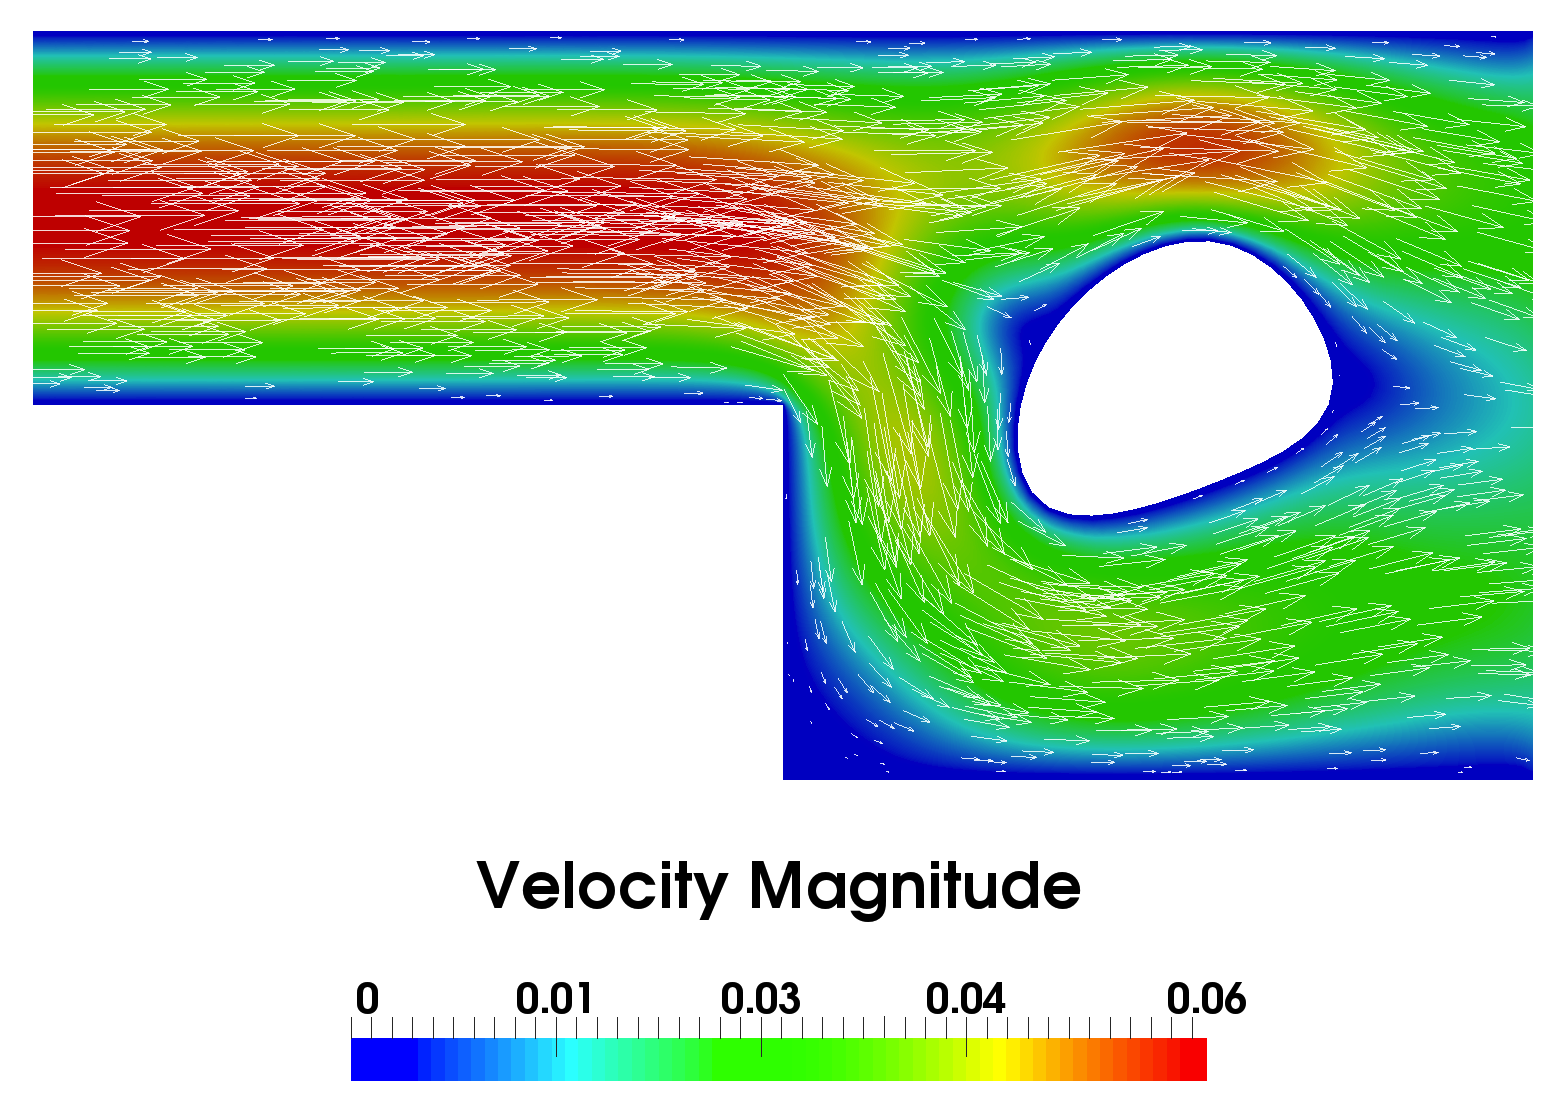
\includegraphics[width=0.7\textwidth]{figures/stokes_gmsh.png}
  \caption{\small Isoviscous Stokes solution for a more complex geometry.
    Boundary conditions are parabolic inflow $u(0,y)=(y-1/2)(1-y),
    v=0$ on the left-hand boundary, Natural outflow boundary
    conditions on the right ($x=2$), and no-flow $\vec{v}=\vec{0}$ on
    all other boundaries including the interior hole.  This example
    uses boundary id's generated by gmsh.}
  \label{fig:stokes_gmsh}
\end{figure}

\subsection{Iterative Solvers and Fieldsplit preconditioners}
\label{sec:iterative-solvers-1}

For moderate sized problems in 2-D, sparse-direct solvers can be
efficient and extremely robust methods.  However, for larger problems
and particularly in 3-D we need to move to iterative solvers.  There
is a large literature on iterative solvers for Stokes equation, 
%% FIXME and future versions of this tutorial will hopefully address
%% at least some of this. 
however, here we will just present one solver for isoviscous
Stokes presented in \cite{elman_finite_2005} as a means of introducing
PETSc's fieldsplit block-preconditioners as implemented in \TF{}.

The discrete inner linear solve in a Newton iteration for Stokes can
be written
\begin{equation}
  \label{eq:21}
     \left[
\begin{array}{cc}
  K & G  \\
  G^{T} & 0 \\
  \end{array}
  \right]
  \left[
    \begin{array}{c}
      \delta \vec{v} \\
      \delta p \\
    \end{array}
  \right] = -\left[
    \begin{array}{c}
      F_{\vec{v}} \\
      F_{p}\\
    \end{array}
  \right]
\end{equation}

May and Moresi \cite{may_preconditioned_2008} present a large number of block
preconditioning schemes for this problem including Schur Complement
Reduction based schemes (SCR) and Fully coupled block preconditioners
(FC).  Here we will discuss one FC upper triangular block
preconditioner
\begin{equation}
  \label{eq:ch3-22}
    \mat{J}_{\text{PC}} =   \left[
\begin{array}{cc}
  K & G  \\
  0 & \hat{S} \\
  \end{array}
  \right]
\end{equation}
where
\begin{displaymath}
  \hat{S} = \int \frac{1}{\eta} p_{t}p dx
\end{displaymath}
is the viscosity weighted pressure mass matrix which has been shown to
be a useful approximation to the Schur Complement $S$ for variable
viscosity problems\cite{grinevich_iterative_2009,ur_rehman_iterative_2011}.  The solution
strategy is to right-precondition the full solution $u=(\vec{v},p)$
with $J_{\text{PC}}$ using a fieldsplit block preconditioner that
first applies an approximate solve to
\begin{equation}
  \hat{S}\delta p = -F_{p}
\label{eq:ch3-23}
\end{equation}
using a lightweight SOR preconditioned CG iterative solver on
$\hat{S}$, then solves
\begin{equation}
  K\delta\vec{v} = -F_{v} - G\delta p
\label{eq:ch3-24}
\end{equation}
using an approximate iterative solve for the viscosity block $K$. In
particular, here we use a second fieldsplit preconditioned iterative
solver for the $K$ block where we use 1 FGMRES iteration on the full
$K$ block, preconditioned by one V-cycle of  an algebraic multi-grid
solver (hypre) on each of the diagonal blocks of $K$. This is
effectively the same pre-conditioner solver used in the RHEA code
\cite{burstedde_large-scale_2013}. Schematically, the tree structure of the nested solver/pre-conditioner set up is shown in
Figure \ref{fig:fieldsplit_stokes}
\begin{figure}[h!]
  \centering 
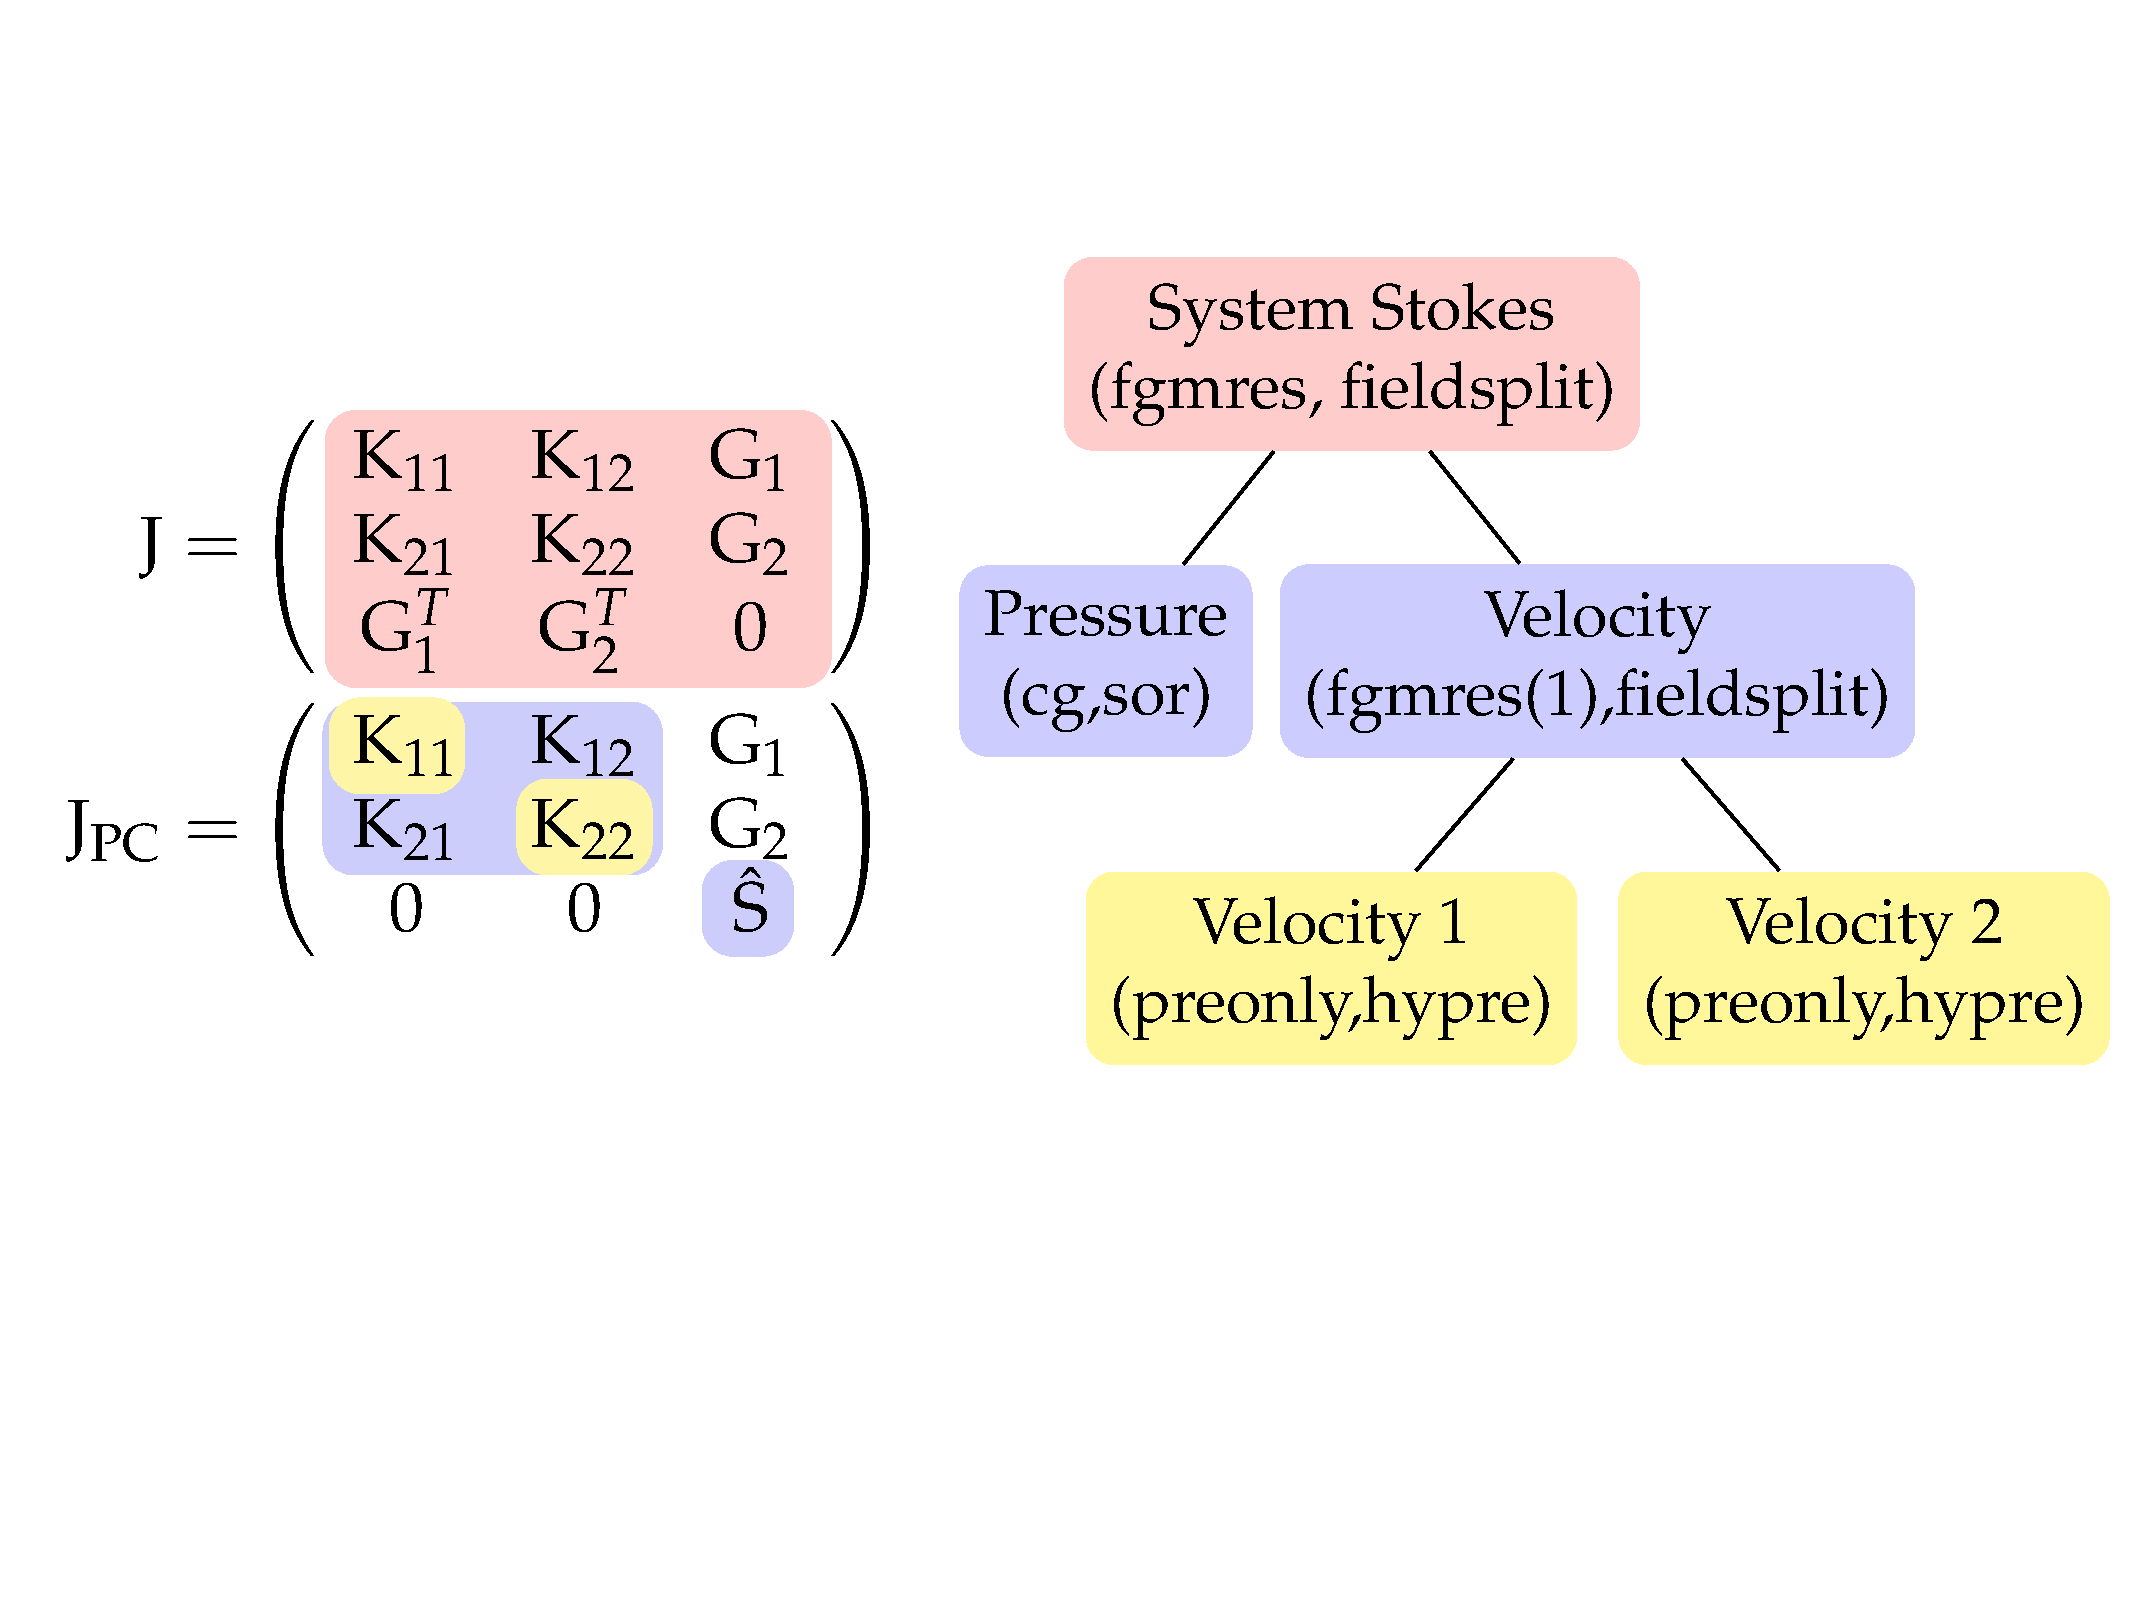
\includegraphics[width=.8\textwidth]{figures/Stokes_block_preconditioners.pdf}
%% way to fragile TikZ stuff here...but useful for making the pdf I
%% eventually used
% \begin{minipage}{0.45\textwidth}
% %\vspace*{-3cm}
% \begin{center}
% \begin{align*}
% \mat{J} =& \left(\begin{array}{ccc}
% \tikzmark{K11}{$\mat{K}_{11}$} & \mat{K}_{12} & \mat{G}_1 \\
% \mat{K}_{21} & \mat{K}_{22} & \mat{G}_2  \\
% \mat{G}_1^T    & \mat{G}_2^T    &  \tikzmark{saddle}{$\mat{0}$}     \\
% \end{array}\right) \\
% \mat{J}_{\text{PC}} = & \left(\begin{array}{ccc}
% \tikzmark{K11PC}{$\mat{K}_{11}$} & \mat{K}_{12} & \mat{G}_1   \\
% \mat{K}_{21} & \tikzmark{K22PC}{$\mat{K}_{22}$} & \mat{G}_2   \\
% \mat{0}    & \mat{0}    & \tikzmark{saddlePC}{$\mat{\hat{S}}$}  \\
% \end{array}\right) \\
% \end{align*}
% \end{center}
% %\vspace*{1cm}
% \end{minipage}
% \hspace{1cm}
% \begin{tikzpicture}[shape=rectangle, rounded corners, align=center,
%     level distance=1.5cm,
%     level 1/.style={sibling distance=2.4cm},
%     level 2/.style={sibling distance=2.6cm}]
%    % level 3/.style={sibling distance=2cm}]
%     % \node [hide on=1, fill=green!20, align=center, font=\footnotesize] {System\\(fgmres, fieldsplit)} [edge from parent fork down]
%     % child [hide on=1] {node [fill=red!20, align=center, font=\footnotesize] {Temperature\\(gmres, ilu)}}
%     \node [fill=red!20, align=center, font=\small] {System Stokes\\(fgmres, fieldsplit)}
%       child  {node [fill=blue!20, align=center, font=\small] {Pressure\\(cg,sor)}}
%       child {node [fill=blue!20, align=center, font=\small] {Velocity\\(fgmres(1),fieldsplit)}
%         child {node [fill=yellow!50, align=center, font=\small] {Velocity 1\\(preonly,hypre)}}
%         child 
%         {node [fill=yellow!50, align=center, font=\small]
%           {Velocity 2\\(preonly,hypre)}}
% };
% \end{tikzpicture}
  \caption{\label{fig:fieldsplit_stokes} Overview of the tree
    structure of nested fieldsplit preconditioners used  for an
    iterative solver for Stokes equation.  $J$ is the expanded
    Jacobian for a 2-dimensional Stokes problem with two-components of
  velocity and pressure.  $J_{\text{PC}}$ is the approximate Jacobian
  used as a pre-conditioner.  At the highest level, we solve $J\delta
  u=-F$ using a pre-conditioned FGMRES scheme (red).  This is
  right pre-conditioned by first solving $J_{\text{PC}}\delta u = -F$
  using $\sim5$ iterations  of (CG,SOR) on the pressure mass matrix
  $\hat{S}$ followed by one iteration of FGMRES on the full $K$ block
  (blue).  The $K$ block is further  preconditioned by a diagonal
  block-preconditioner with one V-cycle of   algebraic multi-grid on
  the diagonal blocks of $K_{11}, K_{22}$ (yellow).}
 \end{figure}

Given the natural tree structure of xml and Spud.  This
nested-fieldsplit preconditioner is relatively straightforward to
describe in \TF{}.  Step-by-Step instructions for modifying the Stokes
MMS problem with a direct solver are as follows (and a fully worked
out example can be found in
\texttt{\$TF\_HOME/share/terraferma/tutorials/stokes/isoviscous/mms/mms\_iterative}.

\begin{steps}{Step}
\item Make a new tfml file from one with a direct solver
  \begin{lstlisting}[style=Bash]
$ mkdir mymms_iterative
$ cd mymms_iterative
$ cp $TF_HOME/share/terraferma/tutorials/stokes/isoviscous/mms/mms_direct/stokes.tfml .
$ diamond stokes.tfml &
  \end{lstlisting}%$
\item \textbf{Remove the reference point in Pressure:} This stokes
  problem is still singular, but we will address it by projecting out
  the null space in the iterative solvers.  So we need to deactivate the
  reference point control tab
  \begin{lstlisting}[style=Python]
    system (Stokes)
       field (Pressure)
         type (Function)
           rank (Scalar)
             reference_point (Point)
  \end{lstlisting}
\item \textbf{Add an additional form for the preconditioner for the
    Jacobian} To implement the upper triangular preconditioner in Eq.\
  (\ref{eq:ch3-22}) we need to add one more form for the preconditioner
  (PETSc, allows passing a separate preconditioning matrix to KSP or
  SNES). Do the following
  \begin{steps}{step}
  \item Under \texttt{nonlinear\_solver
    (Solver)}$\rightarrow$\texttt{type (SNES)} activate the optional
  tab \texttt{form (JacobianPC)} and set the form to the ufl code
  \begin{lstlisting}[style=UFL]
Jpcv = (inner(sym(grad(v_t)), 2.*eta*sym(grad(v_a))) - div(v_t)*p_a)*dx
Jpcp = -p_t*p_a/eta*dx

Jpc = Jpcv + Jpcp
  \end{lstlisting}
Alternatively,  we could be lazy and just recalculate the entire
Jacobian and add the  block $\hat{S}$ using
\begin{lstlisting}[style=UFL]
Jpc = derivative(F,us_i,us_a) - p_t*p_a/eta*dx
\end{lstlisting}
although this will also assemble the $G^{T}$ block.
\item Set the \texttt{ufl\_symbol} to
  \texttt{Jpc}.
\item You might also want to activate and set the
  \texttt{quadrature\_degree} to 3 to keep all the jacobians and
  residuals to the same order of quadrature.
  \end{steps}

\item \textbf{Change the linear solver}.  Now we need to replace the
  direct solver \texttt{(preonly,LU)} with the nested
  fieldsplit-preconditioned fgmres \texttt{(fgmres,fieldsplit)}
  discussed above.  Do the following
  \begin{steps}{step}
  \item Change the iterative solver to \texttt{fgmres} and set the
    following convergence settings:
    \begin{itemize}
    \item restart = 30
    \item relative\_error = 1.e-15
    \item absolute\_error = 1.e-7 (you'll need to activate this but
      this combination of relative and absolute error, makes sure that
      the norm of the residual is reduced to the absolute error, which
      should be somewhat smaller than the truncation error of the MMS
      solution for accuracy.)
    \item max\_iterations = 50
    \item You might also want to turn on \texttt{monitors} for the
      \texttt{preconditioned\_residual}. These will be recorded in the
      log file.  You can also turn on \texttt{convergence\_file} to
      monitor detailed convergence behavior of the solver, but this
      will impact performance.
    \end{itemize}
  \item Change the preconditioner to \texttt{fieldsplit} and do the following
    \begin{enumerate}
    \item \textbf{Set the first fieldsplit (Pressure)}:
      \begin{itemize}
      \item name the first required fieldsplit Pressure
      \item Add a field named Pressure (this name should match that
        given in the system)
      \item Set the linear solver to iterative method (cg) with
        \texttt{relative\_error} 1.e-5 and \texttt{max\_iterations} = 50.
      \item Set the preconditioner to \texttt{(sor)}
      \end{itemize}
    \item \textbf{Set the second fieldsplit (Velocity)}:
      \begin{itemize}
      \item Add a second fieldsplit (named Velocity)
      \item add the field \texttt{Velocity}
        \item Set the linear solver to \texttt{fgmres} with
          \texttt{restart} 30, \texttt{relative\_error} 1.e-3,
          \texttt{max\_iterations} 1
        \item Set the preconditioner to \texttt{fieldsplit}
      \end{itemize}
    \item \textbf{Set additional Fieldsplits for the $K$ block} Here
      we will just use a single hypre algebraic multi-grid cycle on
      each of the diagonal blocks $K_{11}$ and $K_{22}$ in Figure \ref{fig:fieldsplit_stokes}.
      \begin{itemize}
      \item Under this second \texttt{preconditioner (fieldsplit)},
        set the \texttt{composite\_type} to \texttt{(additive)}.  This
        will only do a block-jacobi iteration on the diagonal blocks.\footnote{
        \texttt{composite\_type (multiplicative)} is block
        Gauss-Seidel and acts as either an upper or lower triangular
        block preconditioner depending on the order of the fields in
        the Jacobian and of the splits. \texttt{composite\_type
          (additive)} is a block-diagonal preconditioner.}
      \item Name the first fieldsplit Velocityx.
      \item Set the field name to \texttt{Velocity}
      \item add the \texttt{components} tab and set the component to 0
        (horizontal velocity)
      \item Set the \texttt{linear\_solver} for this fieldsplit to
        \texttt{(preonly,hypre)}
      \item Add a second fieldsplit for \texttt{Velocityy} (or use the
        copy/paste function in diamond to copy \texttt{Velocityx}.
      \item Repeat the above procedure but set \texttt{components} to 1.
      \end{itemize}
    \end{enumerate}
  \item \texttt{Remove the pressure Null space in the solver}: Under
    the top level \texttt{linear\_solver}, \texttt{(fgmres,fieldsplit)}, we need
    to remove the null-space associated with a constant pressure mode.
    \begin{enumerate}
    \item Activate the \texttt{remove\_null\_space} tab under the
      top-level \texttt{linear\_solver}.
    \item Name the \texttt{null\_space} \texttt{ConstantPressure}
    \item Under \texttt{null\_space} activate the field and name it \texttt{Pressure}
    \item Make sure the null space is set to \texttt{constant} (for
      more complicated spaces you can also provide a python routine to
      calculate the null-space)
    \end{enumerate}
  \end{steps}
\item \texttt{Make and run the program}
  \begin{lstlisting}[style=bash]
$ tfbuild stokes.tfml
$ cd build
$ make -j 2 
$ make run
\end{lstlisting}


\end{steps}

That should do it.  

\subsubsection{Replacing python expressions with C++ expressions}

While convenient, using python to evaluate expressions can be
expensive for large problems and also has the issue that python does
not share a name-space with dolfin and ufl and cannot always share or
use other derived functions.  For this reason, we also allow you to
directly overload the C++ Expressions from dolfin.  A full description
of the process is beyond the current scope of these tutorials, but
simplified examples are given in all the \texttt{.tfml} files in the
subdirectory \texttt{compare\_solvers}. Changing from
python to C++ expressions improves the overall run-time if python is
heavily used in the diagnostics (e.g. an estimate of the L2 norm of
the error against the manufactured solution) but has only minimal
impact on the solver and assembly time if python is only involved in
setting boundary conditions.

\subsubsection{Solver comparison}
\label{sec:solver-comparison}

Figure \ref{fig:stokes_solver_convergence_timing}  shows convergence
and timing results for three different stokes solvers available under
\texttt{\$TF\_HOME/share/terraferma/tutorials/stokes/isoviscous/mms/compare\_solvers}.
\begin{itemize}
\item \texttt{mms\_direct} uses a sparse-direct solver on the full Jacobian
\item \texttt{mms\_iterative} uses the nested fieldsplit iterative
  scheme described above
\item \texttt{mms\_fs\_direct} uses the same upper-triangular block
  preconditioner but uses a sparse direct solver on each of the
  $\hat{S}$ and $K$ blocks.
\end{itemize}
These plots can be reproduced by running
\begin{lstlisting}[style=Bash]
   $ cd $TF_HOME/share/terraferma/tutorials/stokes/isoviscous/mms/compare_solvers
   $ . ./environment
   $ tfsimulationharness --test compare_solvers.py 
 \end{lstlisting} %$
 (see the \texttt{README} file for more details).
These examples only show a few of the possible configurations of
solvers and preconditioners possible for Stokes under
TF. Nevertheless,  they demonstrate that optimal solvers can be
readily constructed and tested in TF.  


\begin{figure}[htbp!]
  \centering
 \textbf{a} 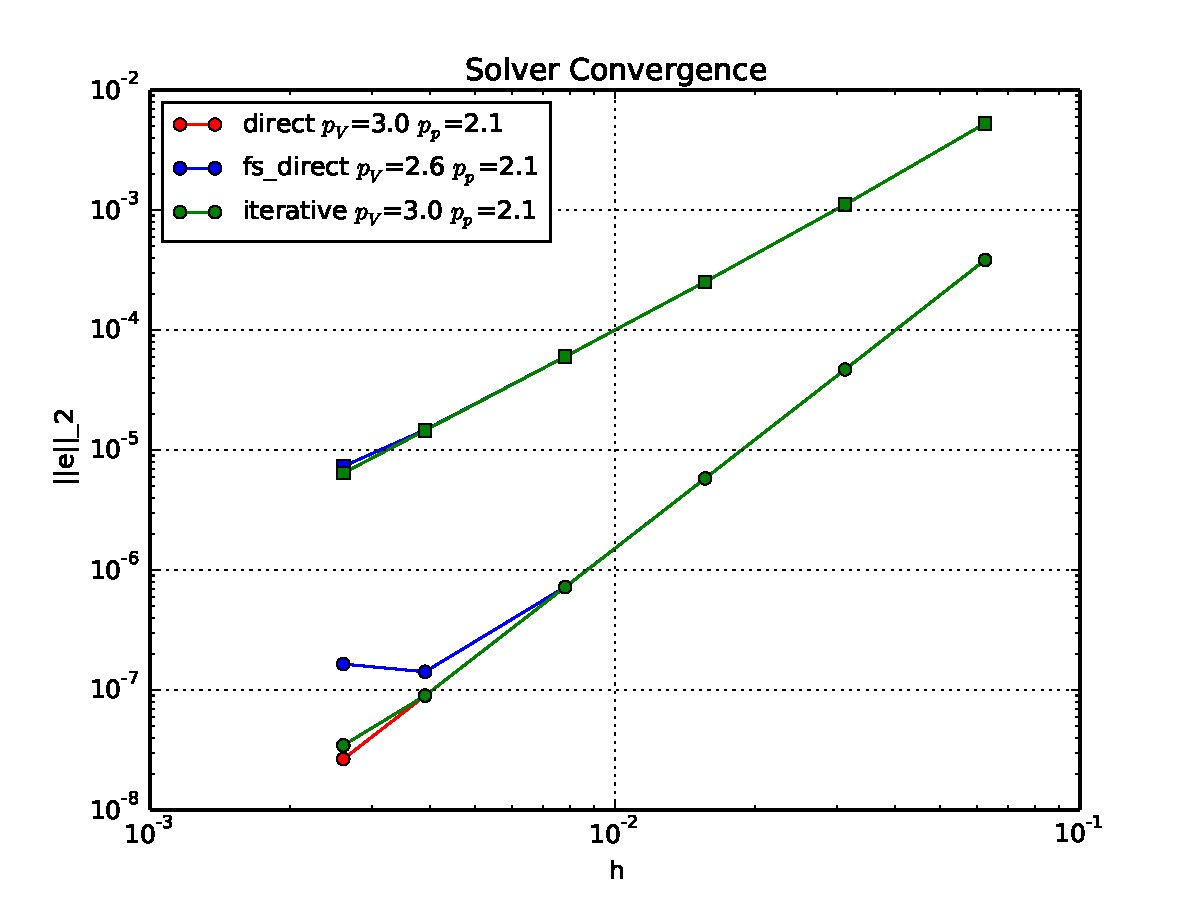
\includegraphics[width=.65\textwidth]{figures/Solver_comparison_convergence.pdf}\\
\textbf{b}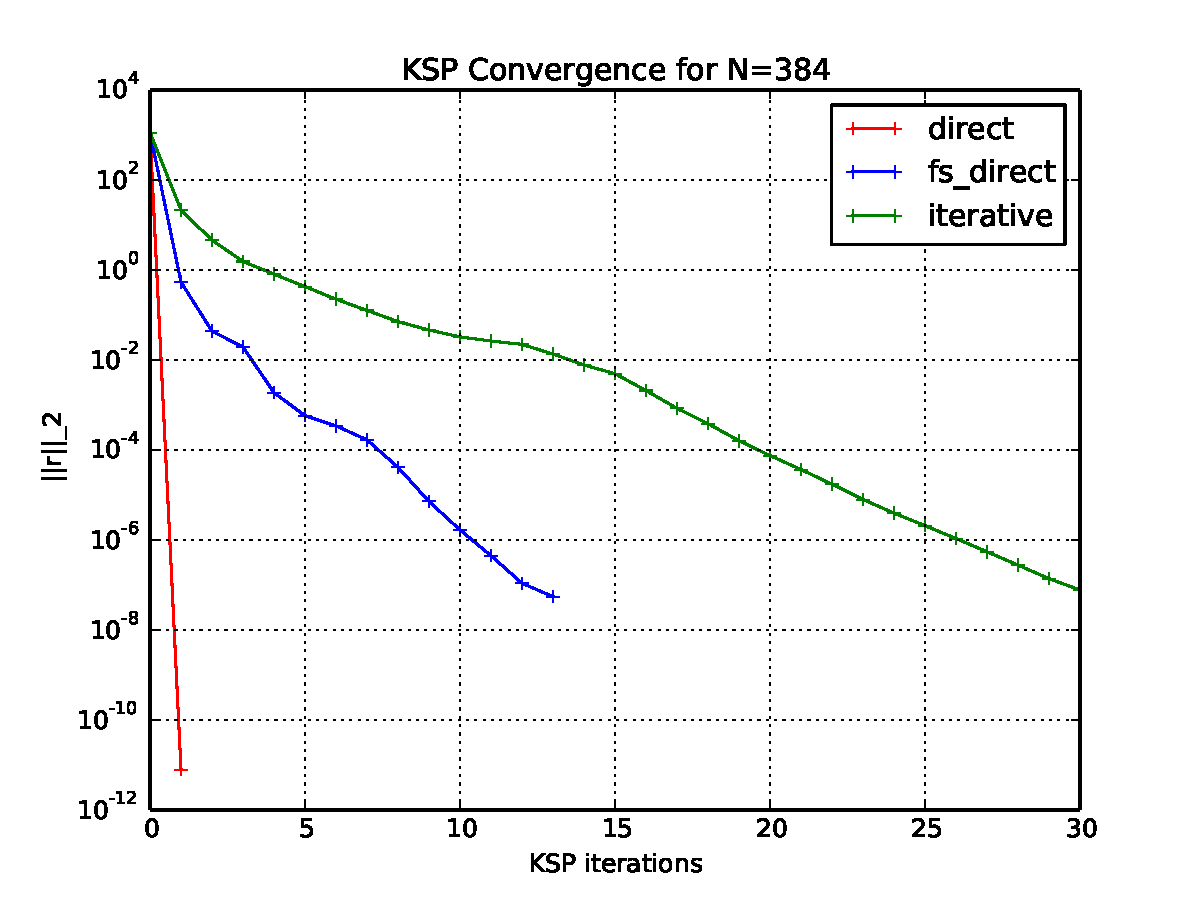
\includegraphics[width=.65\textwidth]{figures/Solver_Comparison_ksp_convergence.pdf}\\
\textbf{c}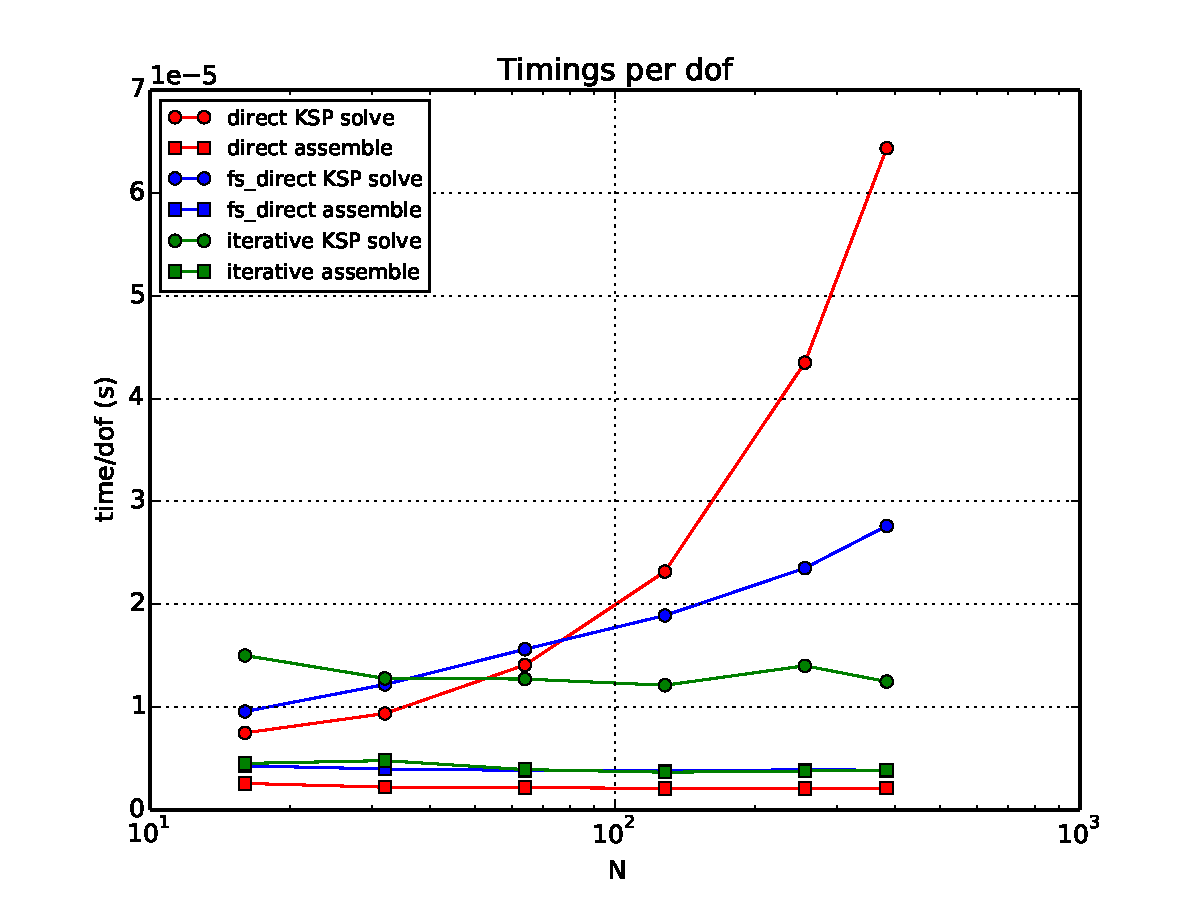
\includegraphics[width=.65\textwidth]{figures/Solver_Comparison_normalized_solver_timing.pdf}\\
  \caption{Comparison of Convergence and performance of MMS solution
    for three different solvers.  (\textbf{a}) relative error of
    solutions with respect to exact solution. (\textbf{b}) convergence behavior
    of the different linear solvers with respect to  the non-linear
    residual. (\textbf{c}) Performance.  Assembly and solver-time per
    degree of freedom.  Note increased assembly time for fieldsplit
    preconditioners reflects assembly of a second jacobian.
    \texttt{mms\_iterative} is optimal in that the timing scales only
    with $N$.}
  \label{fig:stokes_solver_convergence_timing}
\end{figure}

%%% Local Variables: 
%%% mode: latex
%%% TeX-master: "tftutorials"
%%% End: 
